% \begin{frame}{Runwise Plots}
%     \begin{itemize}
%         \item Various changes during runs
%         \item NTracks/Lumi
%         \item Nevent/Lumi
%     \end{itemize}
% \end{frame}

\begin{frame}{2024 Runs Splits}
    \begin{itemize}
        \item Due to the higher backgrounds FaserNu had to be replaced every 10 ifb.
        \item The replacement schedule was as follows
    \end{itemize}
    \begin{table}[h!]
        \begin{tabular}{|l|c|c|c|}
            \hline
            \textbf{Box}  & \textbf{Installed} & \textbf{Removed} & \textbf{Lumi (ifb)} \\ \hline
            F241          & 20/3               & 6/5              & 11.6                \\ \hline
            Tungsten only & 6/5                & 12/6             & 18.5                \\ \hline
            F242          & 12/6               & 8/7              & 9.9                 \\ \hline
            CaloNu        & 10/7               & 4/10             & 69.8                \\ \hline
            F243          & 4/10               & 22/10            & 11.9                \\ \hline
        \end{tabular}
        \caption{Replacement Schedule [Source: \href{https://indico.cern.ch/event/1350805/contributions/5686417/attachments/2963344/5212652/FASER-GeneralMtg-8.11.24.pdf}{FASER General Meeting 8.11.24}]}
    \end{table}
    \begin{itemize}
        \item The runs are split into categories based on the above schedule
        \item Allowed a construction of Yield plots for each category, NEvents/Lumi (Top) and NTracks/Lumi (Bottom)
    \end{itemize}
    \scriptsize{Note: Run numbers are estimated from the schedule and aforementioned run-list thus, it may not be accurate or complete.}
\end{frame}

\begin{frame}{Yield Plots of 2023}
    \begin{figure}
        \centering
        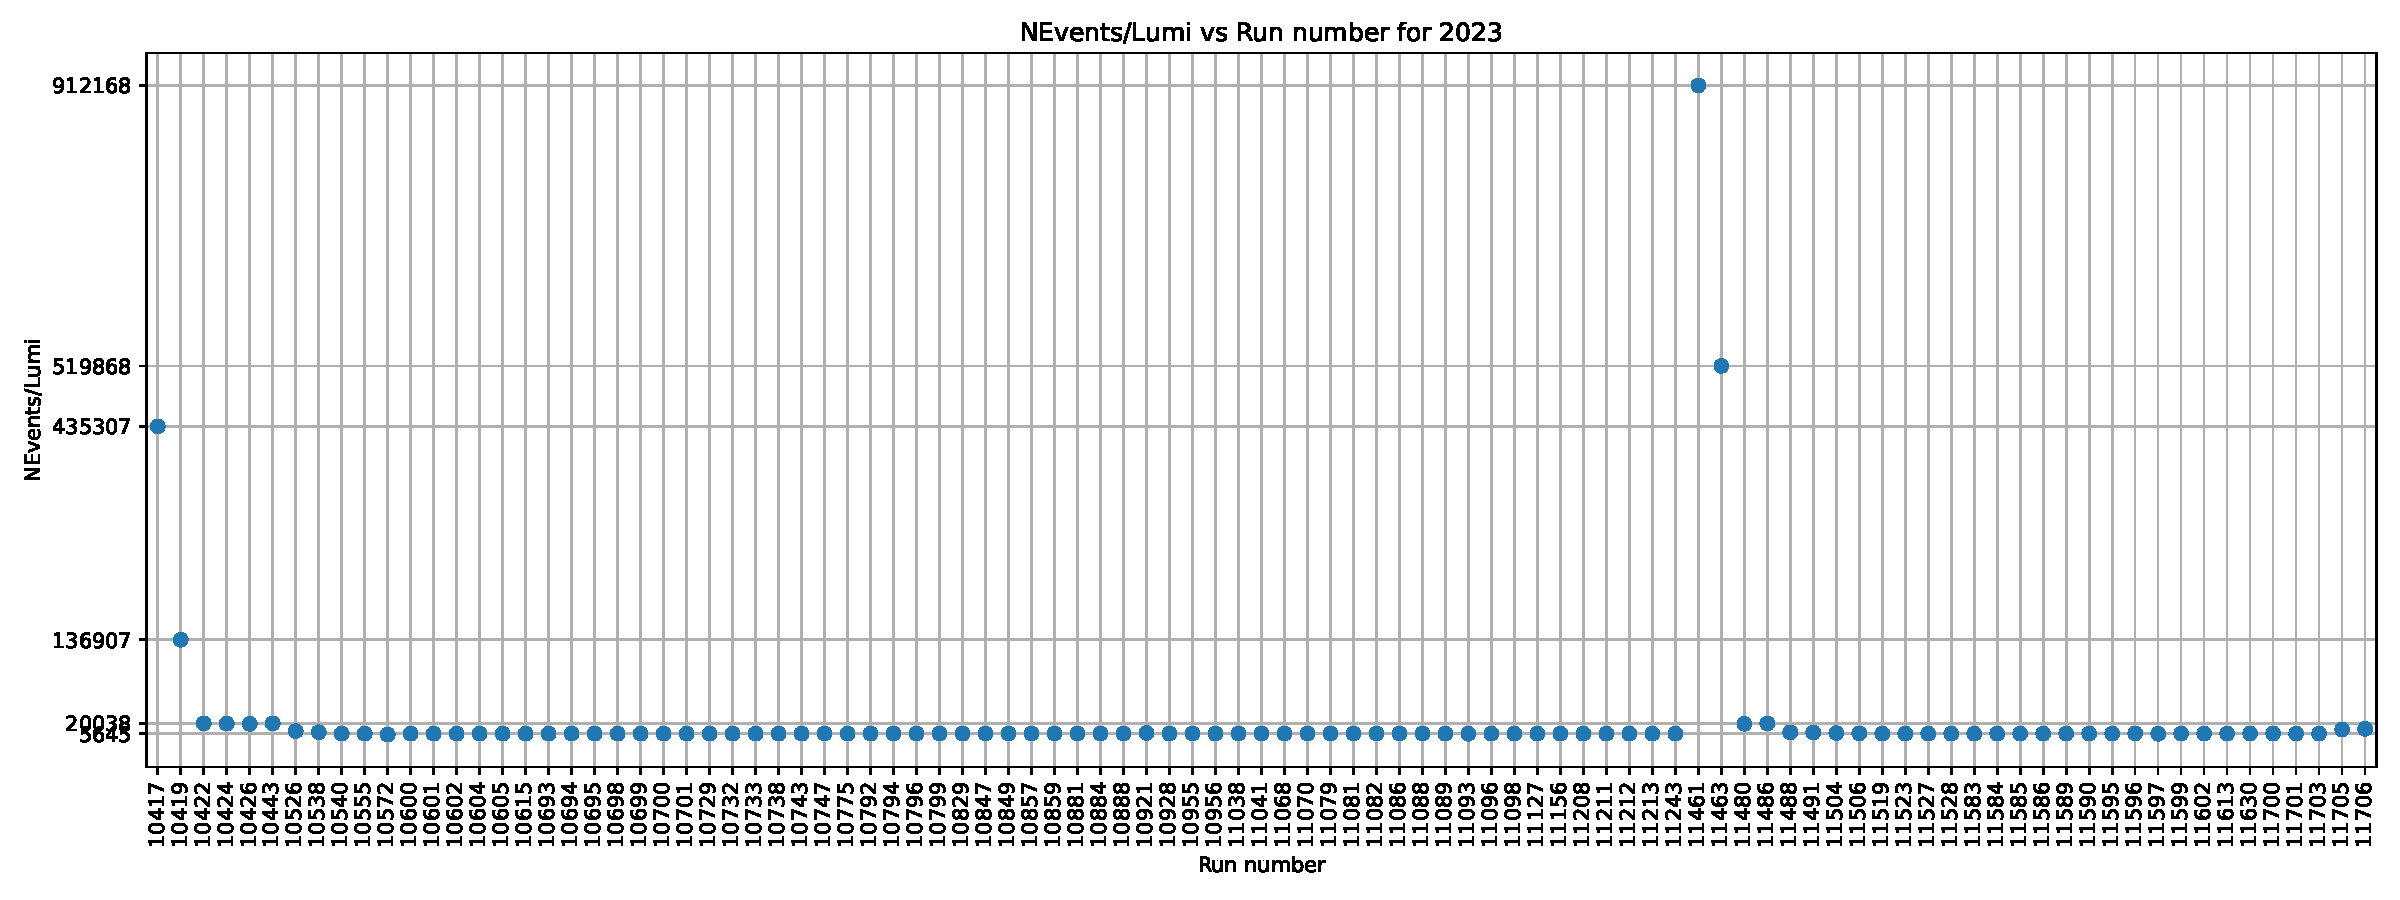
\includegraphics[width=1.0\textwidth]{plots_runwise/NEventsbyLumi_2023.pdf}
    \end{figure}
    \vspace{-0.35cm}
    \begin{figure}
        \centering
        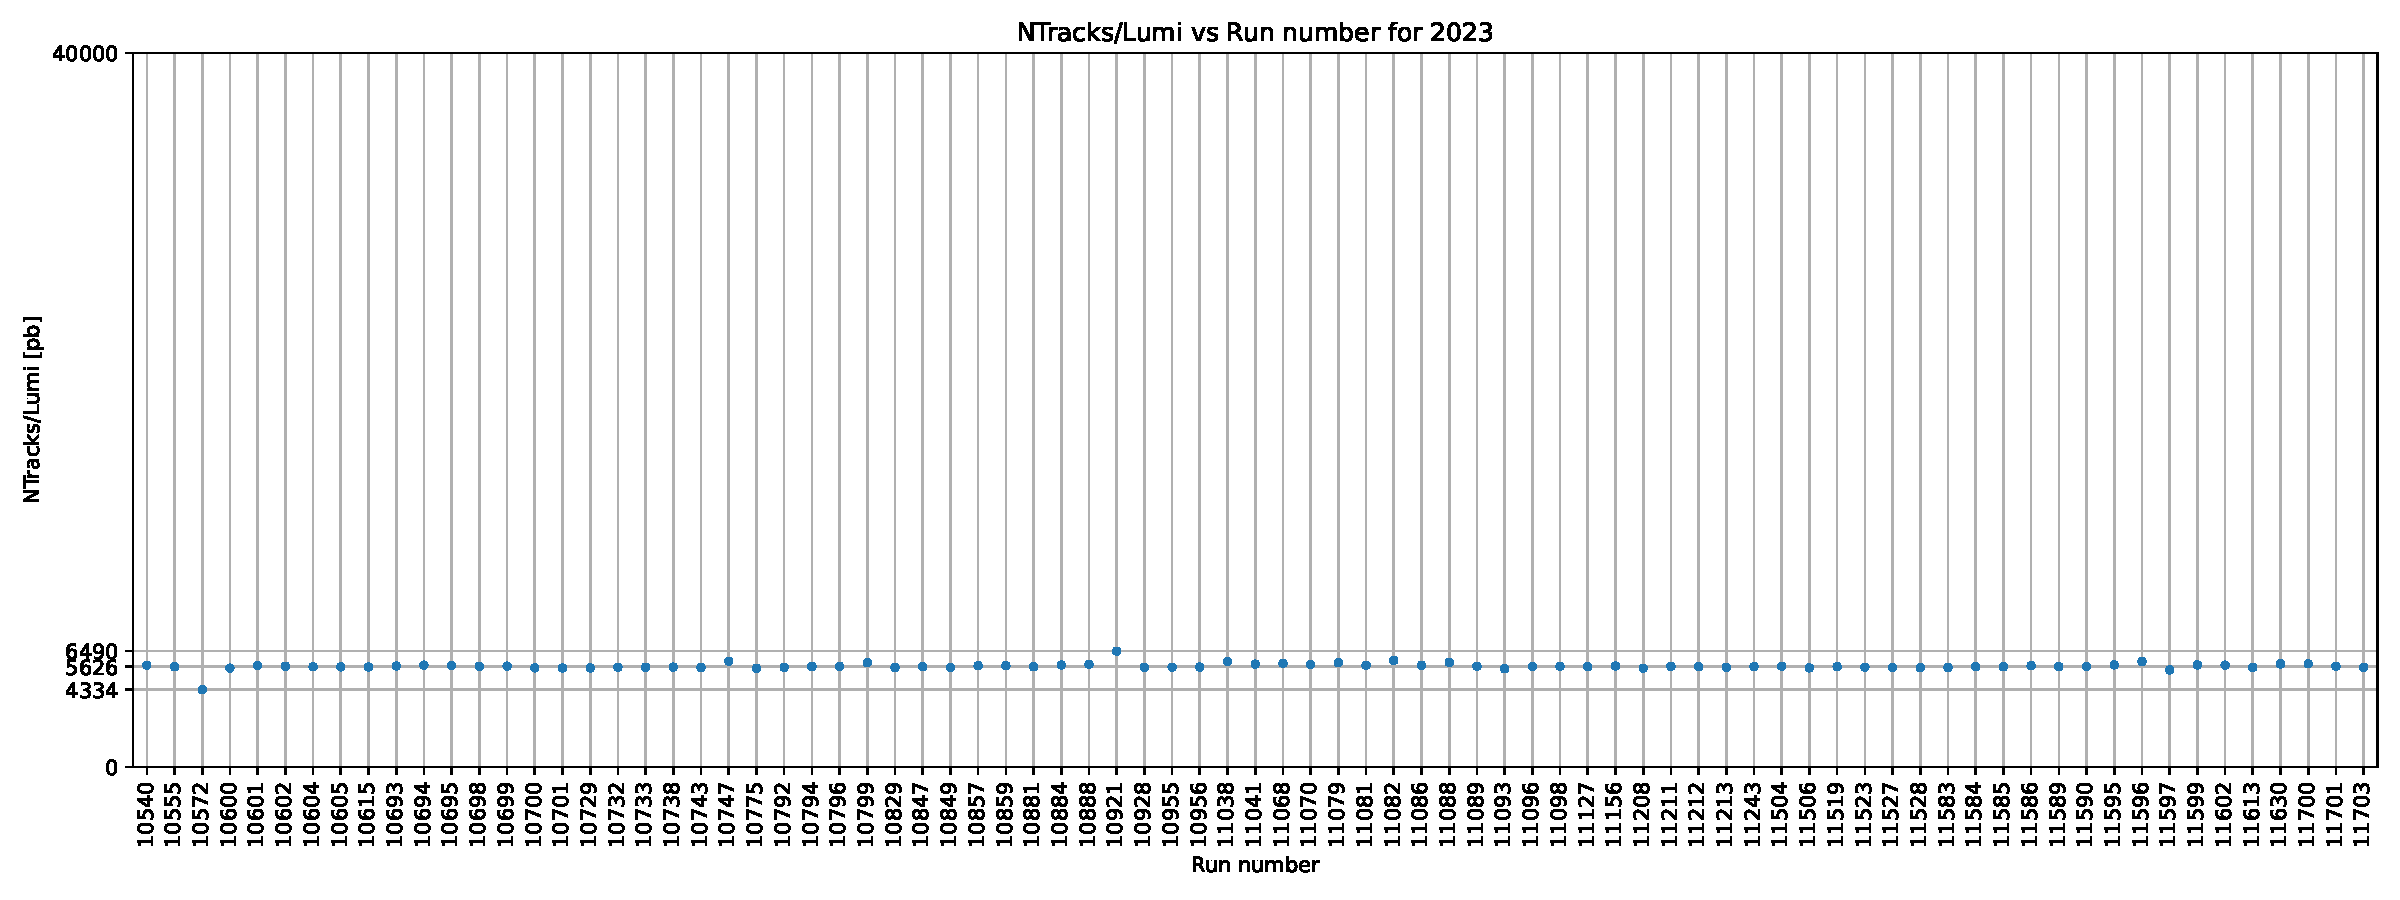
\includegraphics[width=1.0\textwidth]{plots_runwise/NTracksbyLumi_2023.pdf}
    \end{figure}
\end{frame}



\begin{frame}{Yield Plots of F241- 2024}
    \begin{figure}
        \centering
        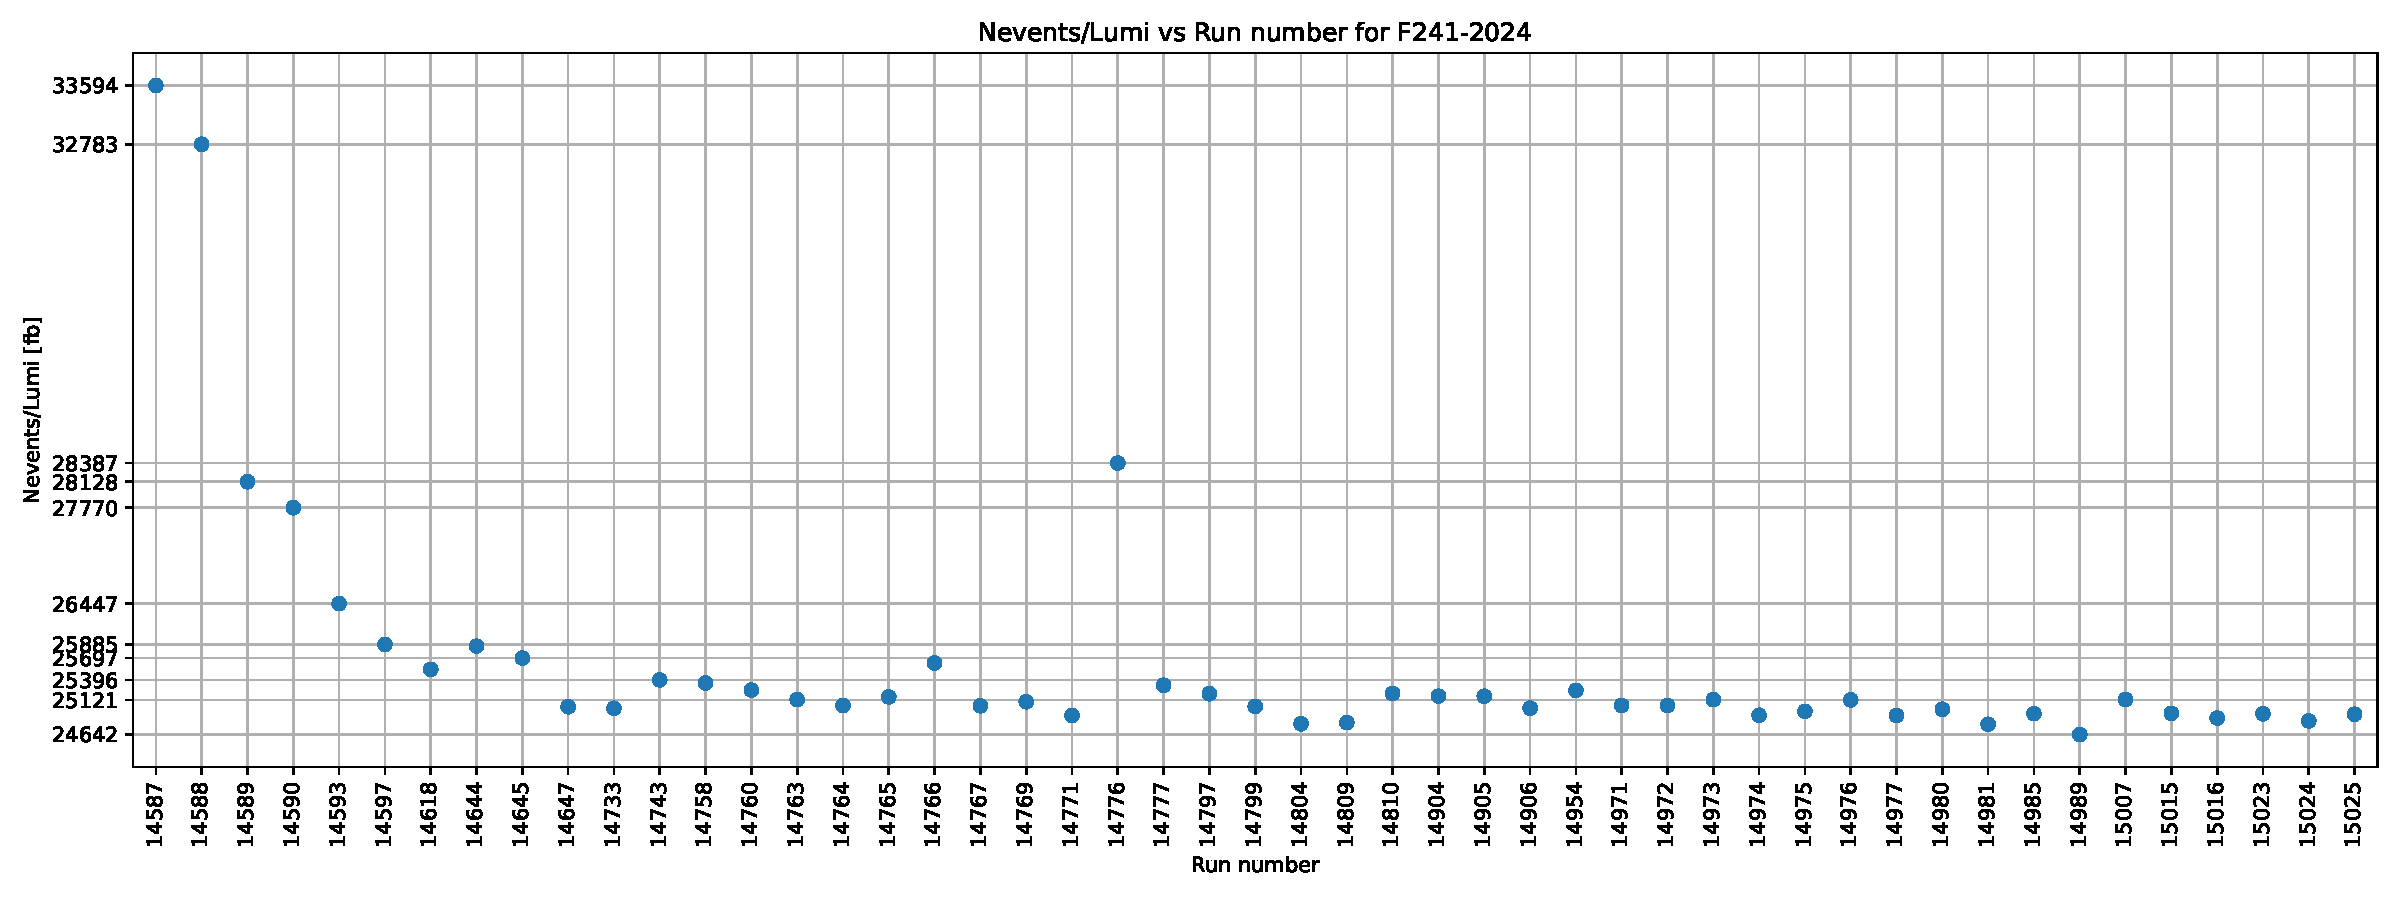
\includegraphics[width=1.0\textwidth]{plots_runwise/NEventsbyLumi_2024_F241.pdf}
    \end{figure}
    \vspace{-0.35cm}
    \begin{figure}
        \centering
        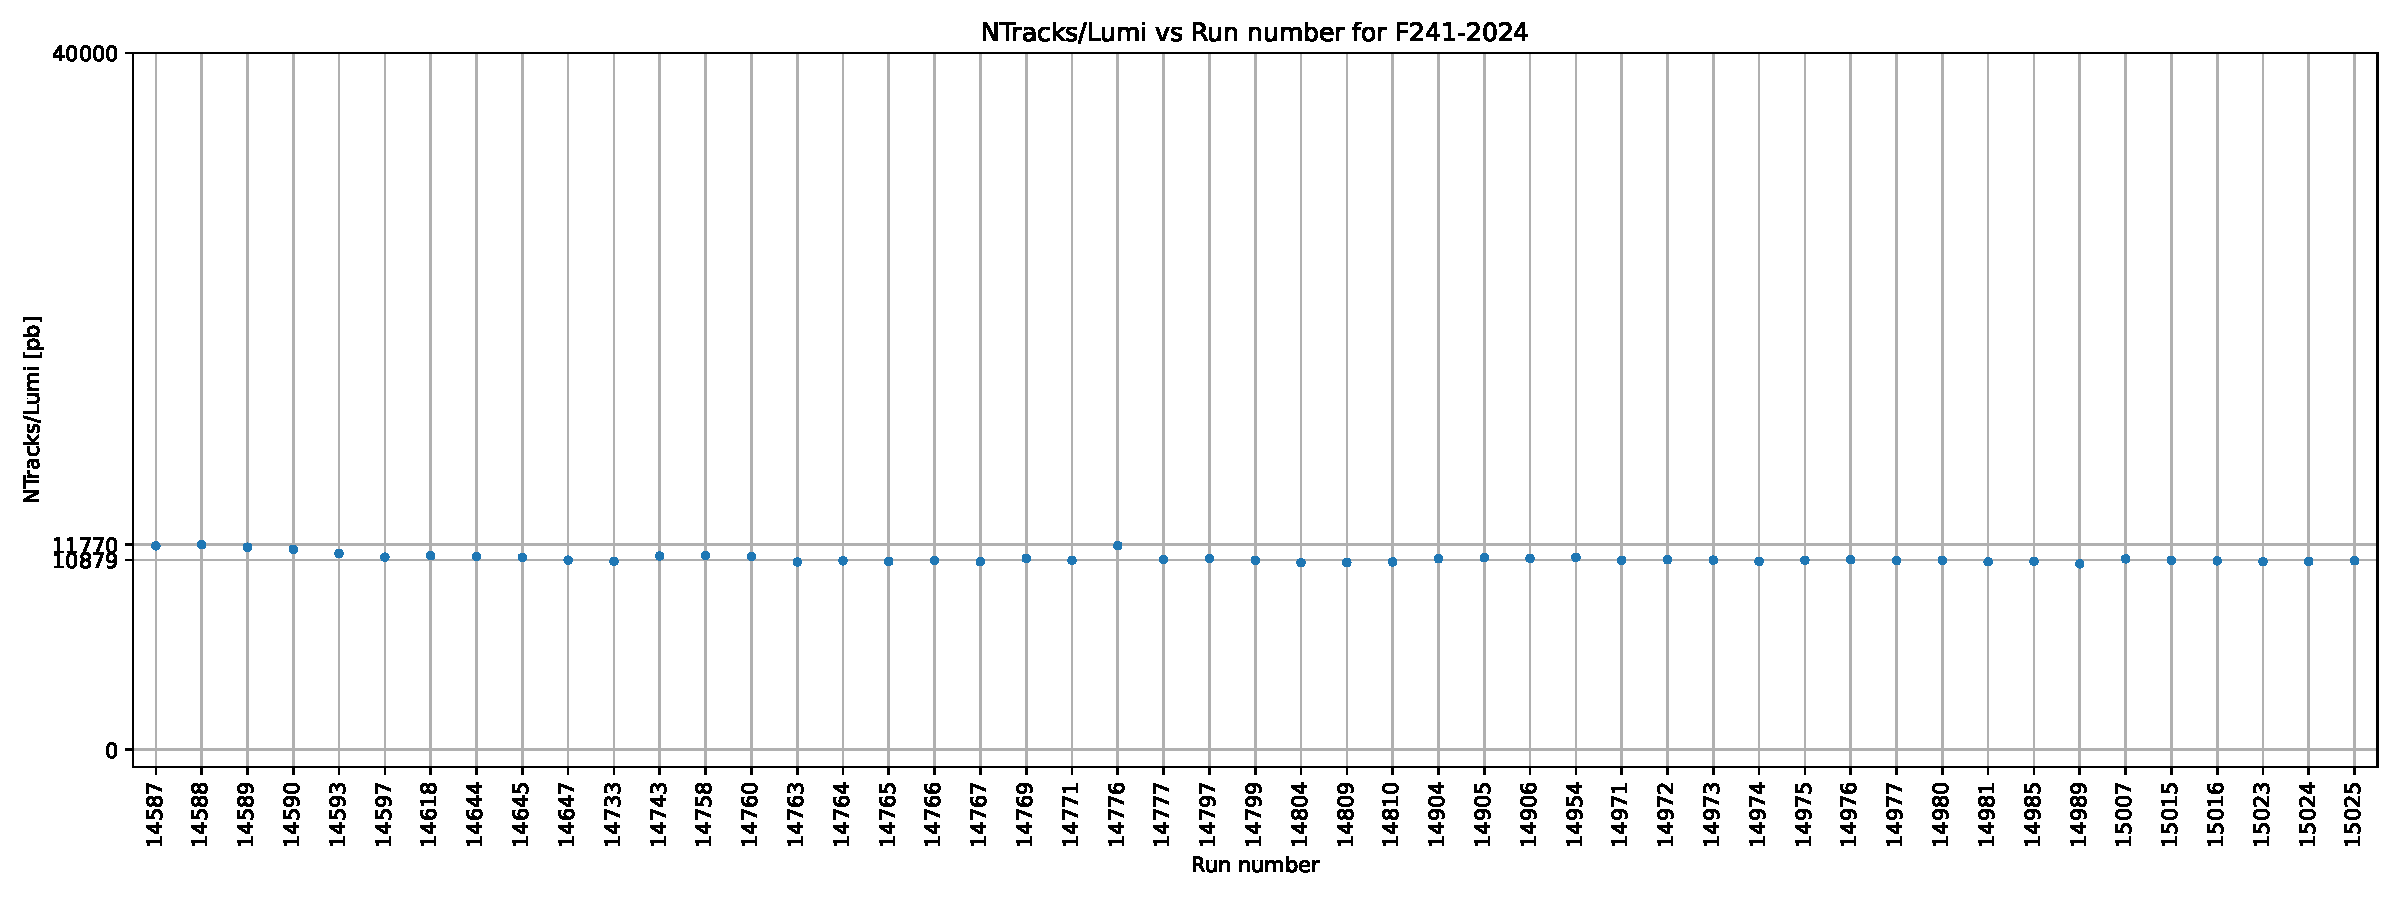
\includegraphics[width=1.0\textwidth]{plots_runwise/NTracksbyLumi_2024_F241.pdf}
    \end{figure}
\end{frame}

\begin{frame}{Yield Plots of Tungsten only- 2024}
    \begin{figure}
        \centering
        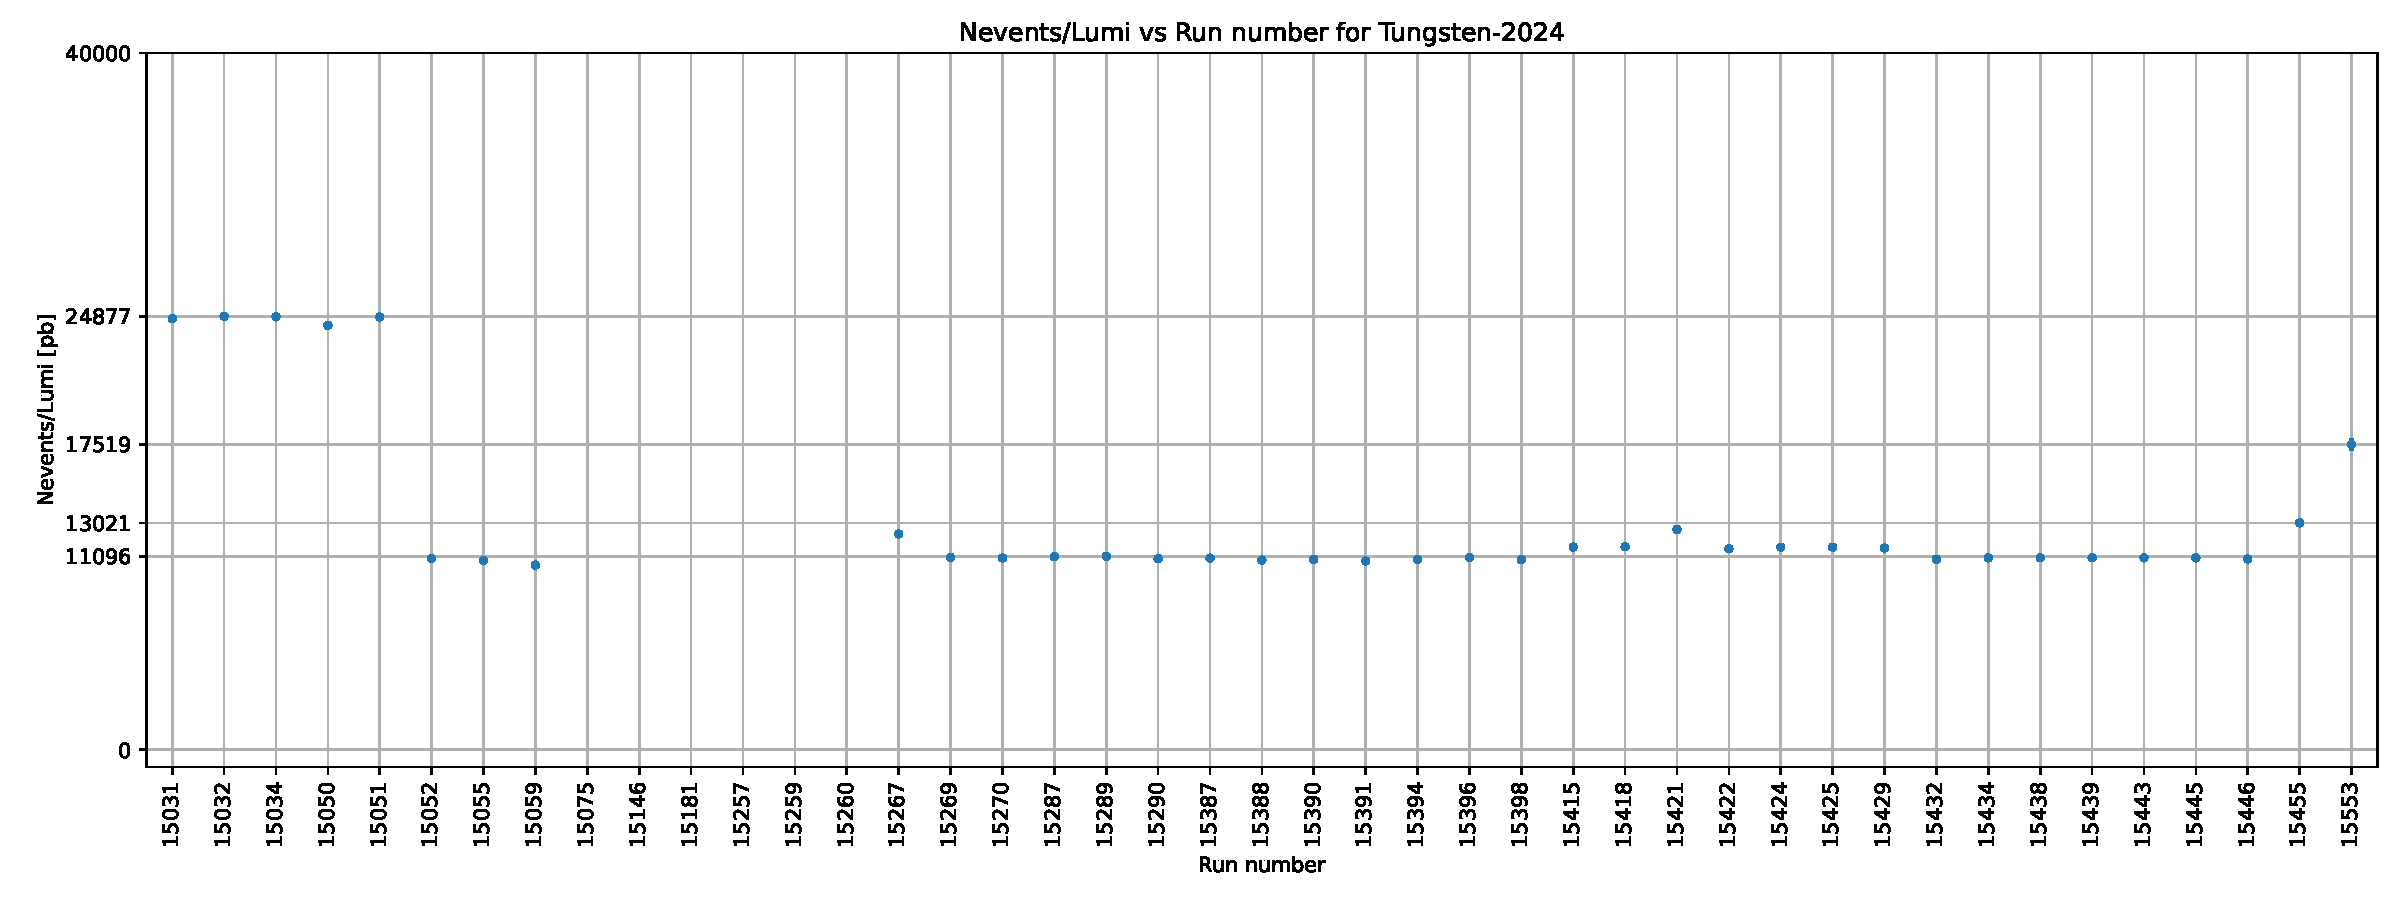
\includegraphics[width=1.0\textwidth]{plots_runwise/NEventsbyLumi_2024_Tungsten.pdf}
    \end{figure}
    \vspace{-0.35cm}
    \begin{figure}
        \centering
        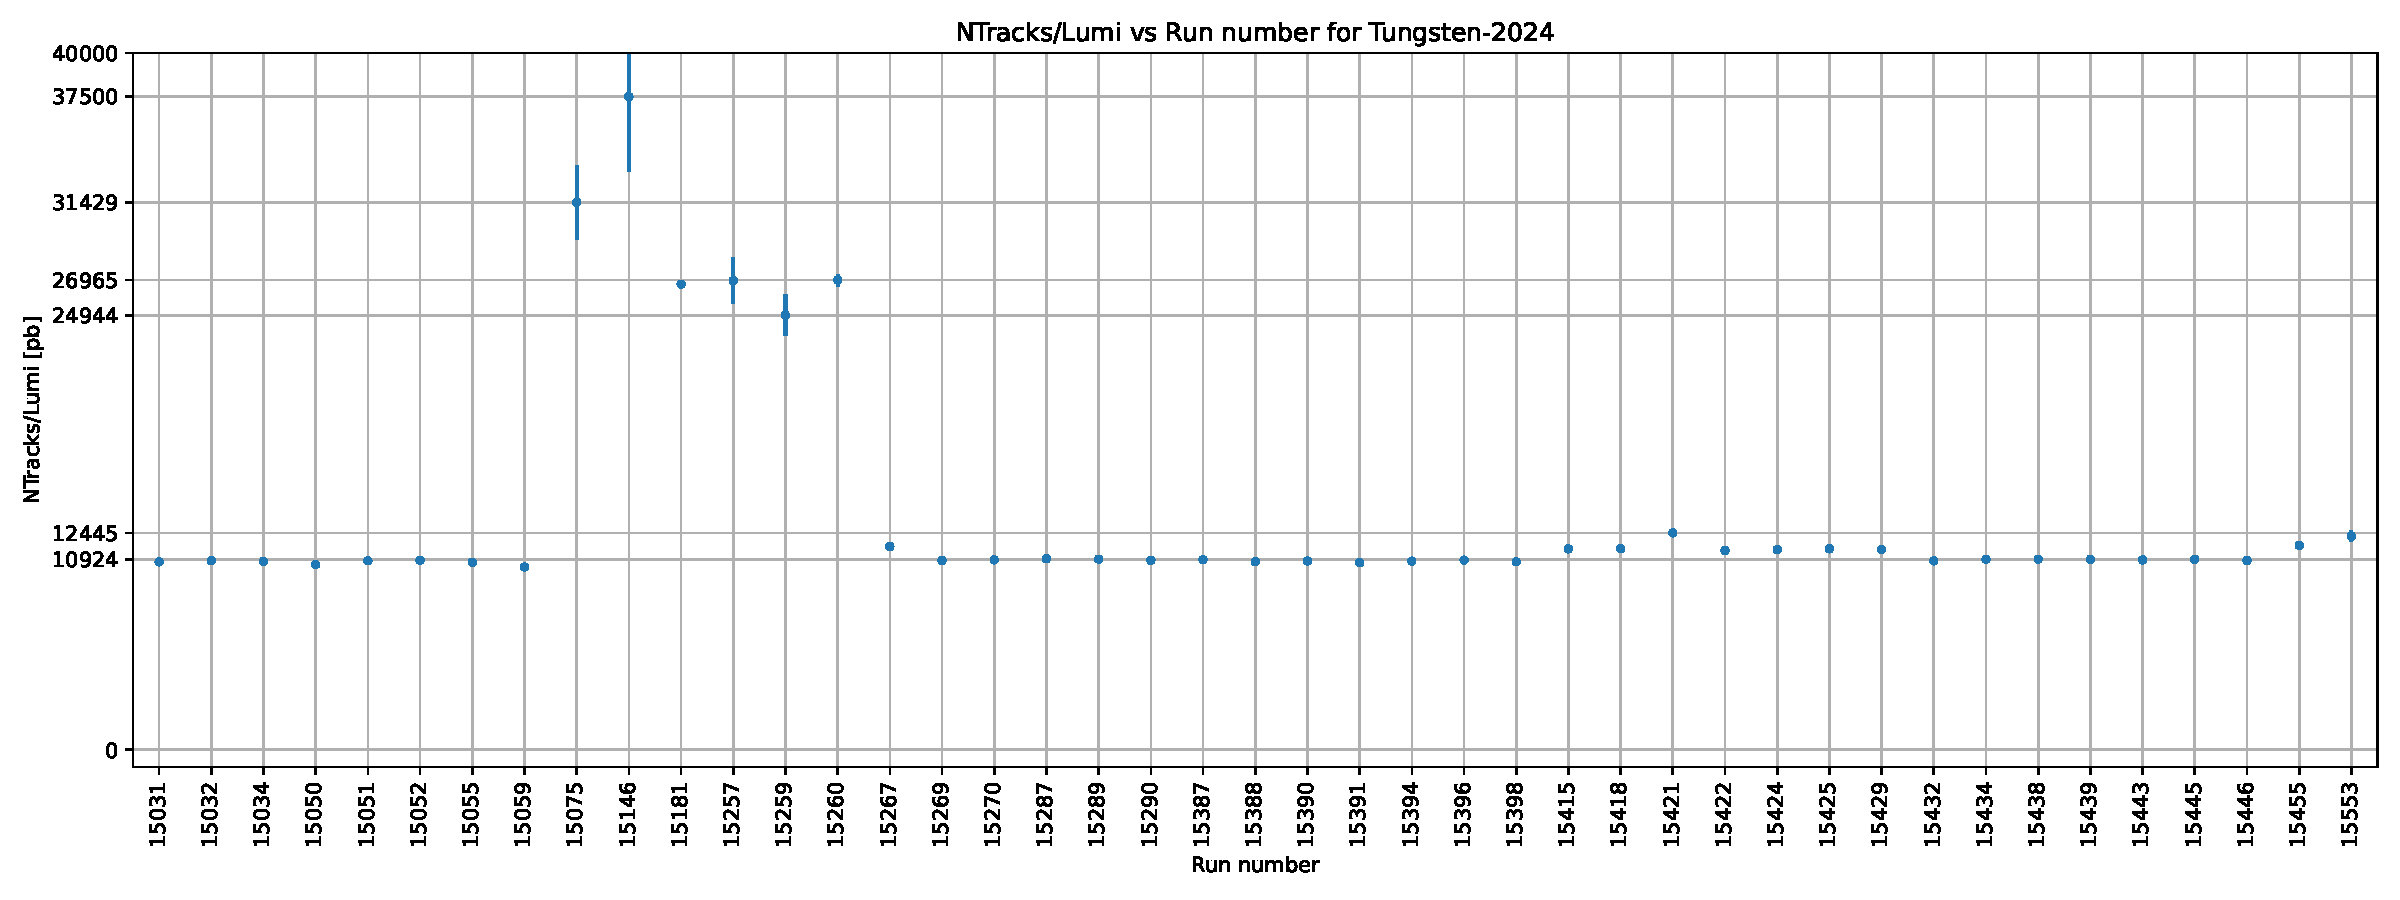
\includegraphics[width=1.0\textwidth]{plots_runwise/NTracksbyLumi_2024_Tungsten.pdf}
    \end{figure}
\end{frame}

\begin{frame}{Yield Plots of F242- 2024}
    \begin{figure}
        \centering
        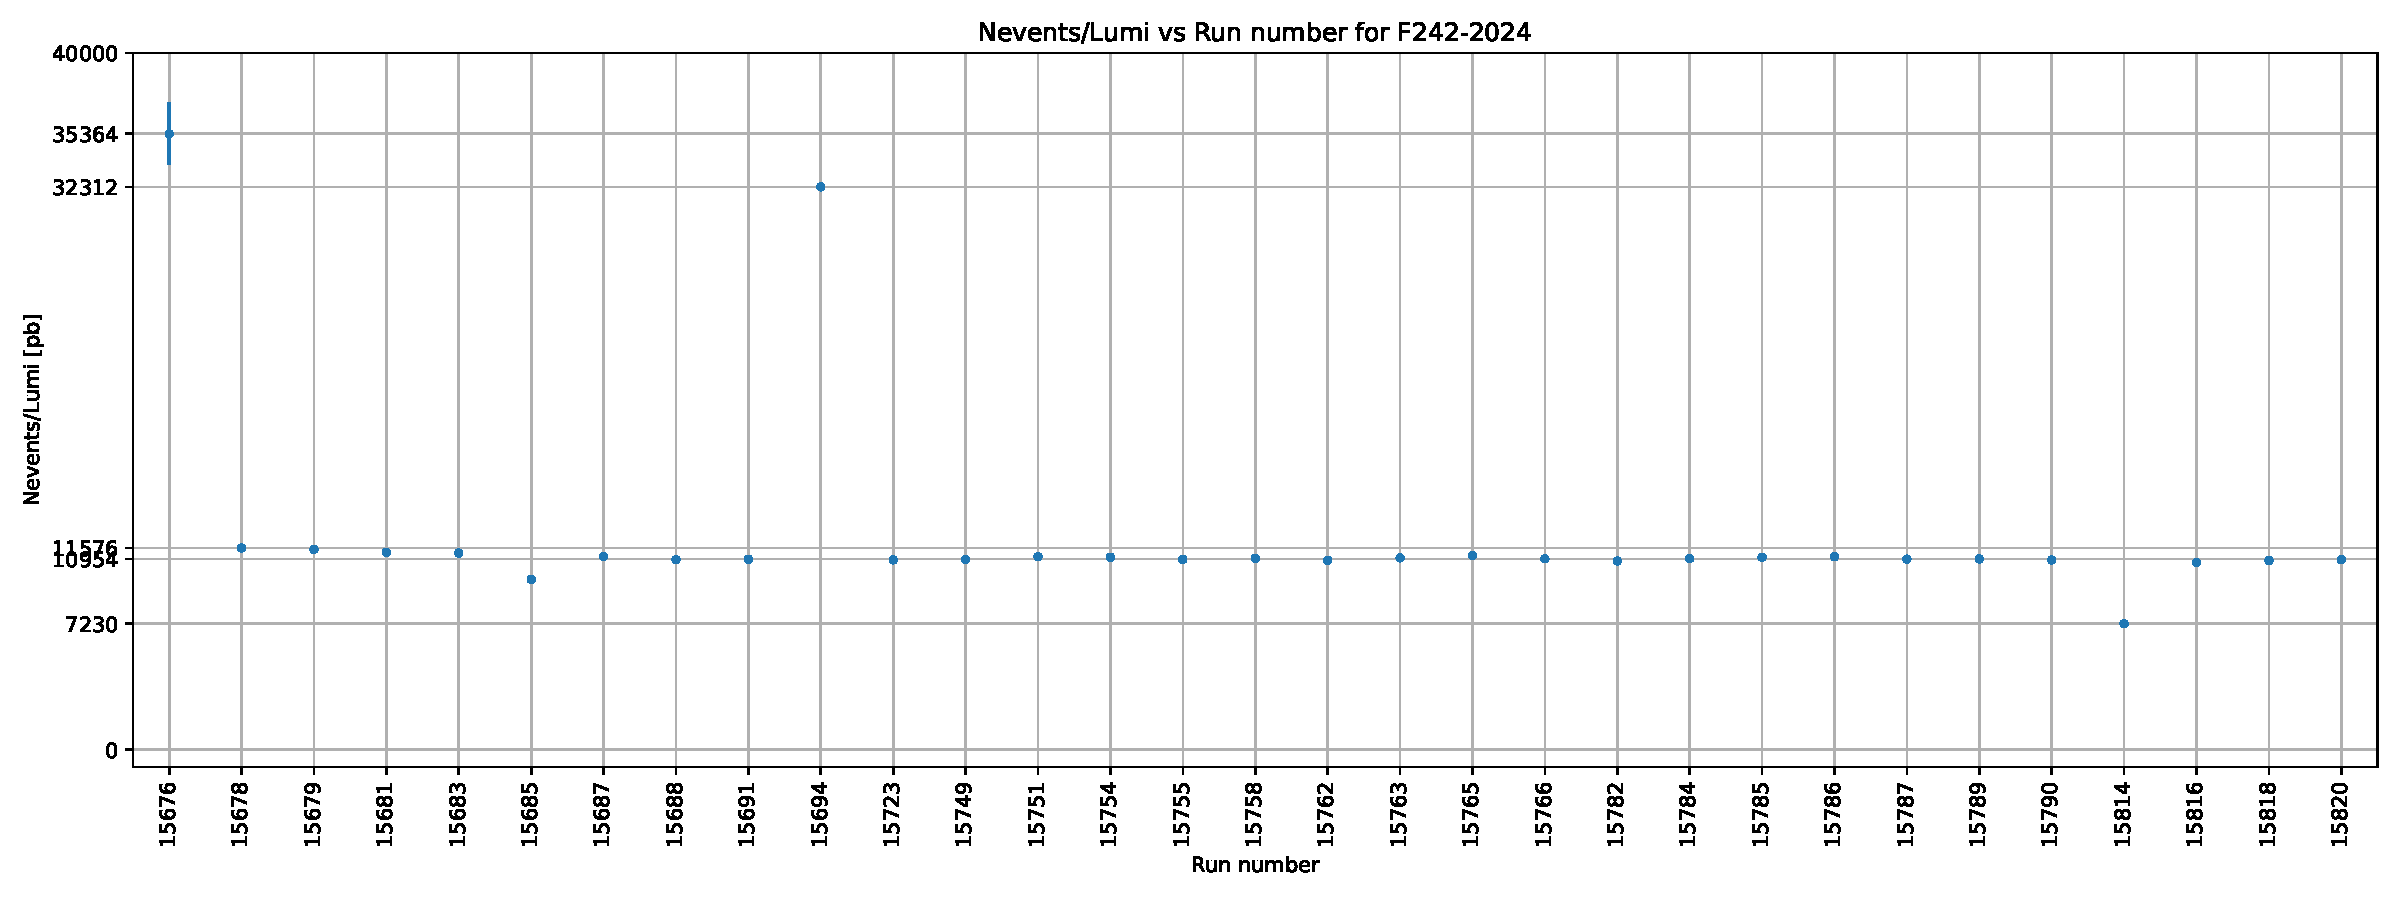
\includegraphics[width=1.0\textwidth]{plots_runwise/NEventsbyLumi_2024_F242.pdf}
    \end{figure}
    \vspace{-0.35cm}
    \begin{figure}
        \centering
        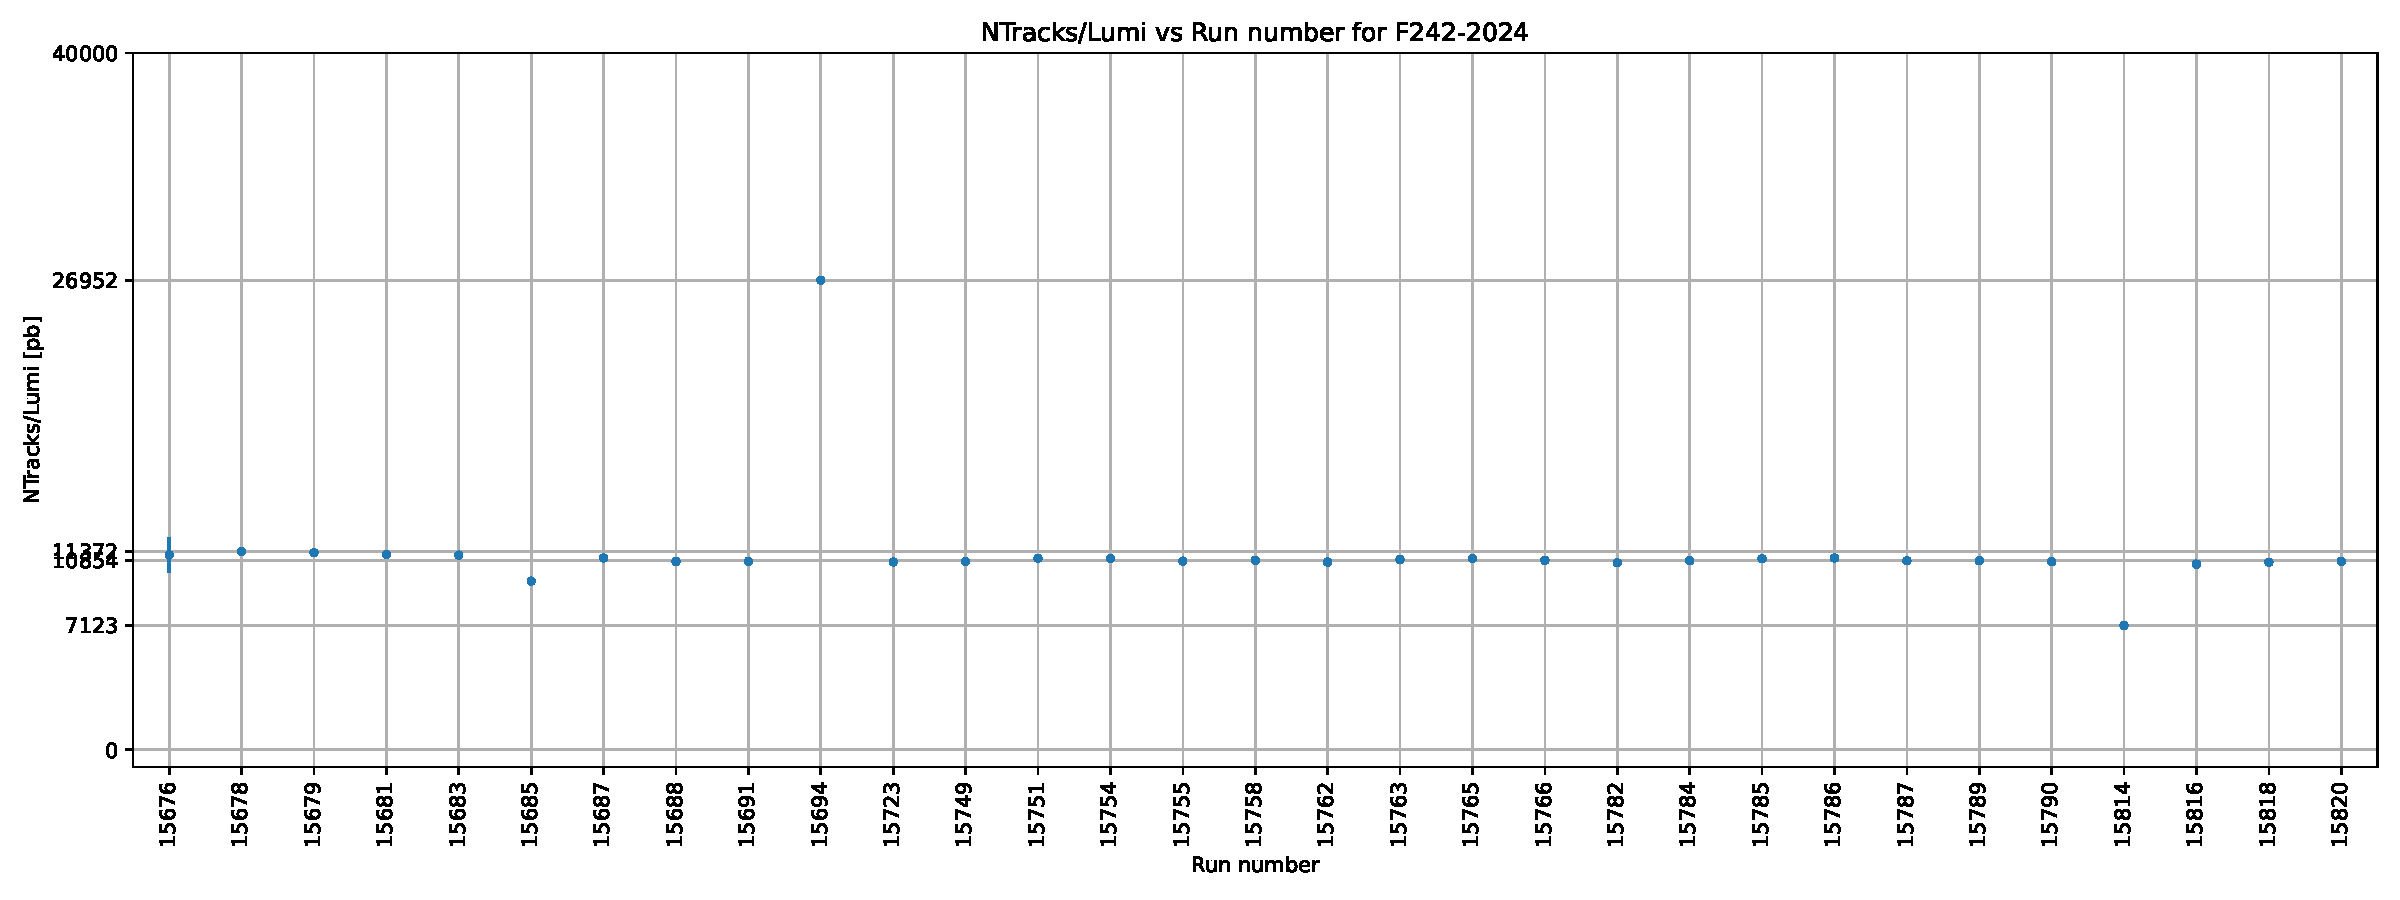
\includegraphics[width=1.0\textwidth]{plots_runwise/NTracksbyLumi_2024_F242.pdf}
    \end{figure}
\end{frame}

\begin{frame}{Yield Plots of CaloNu - 2024}
    \begin{figure}
        \centering
        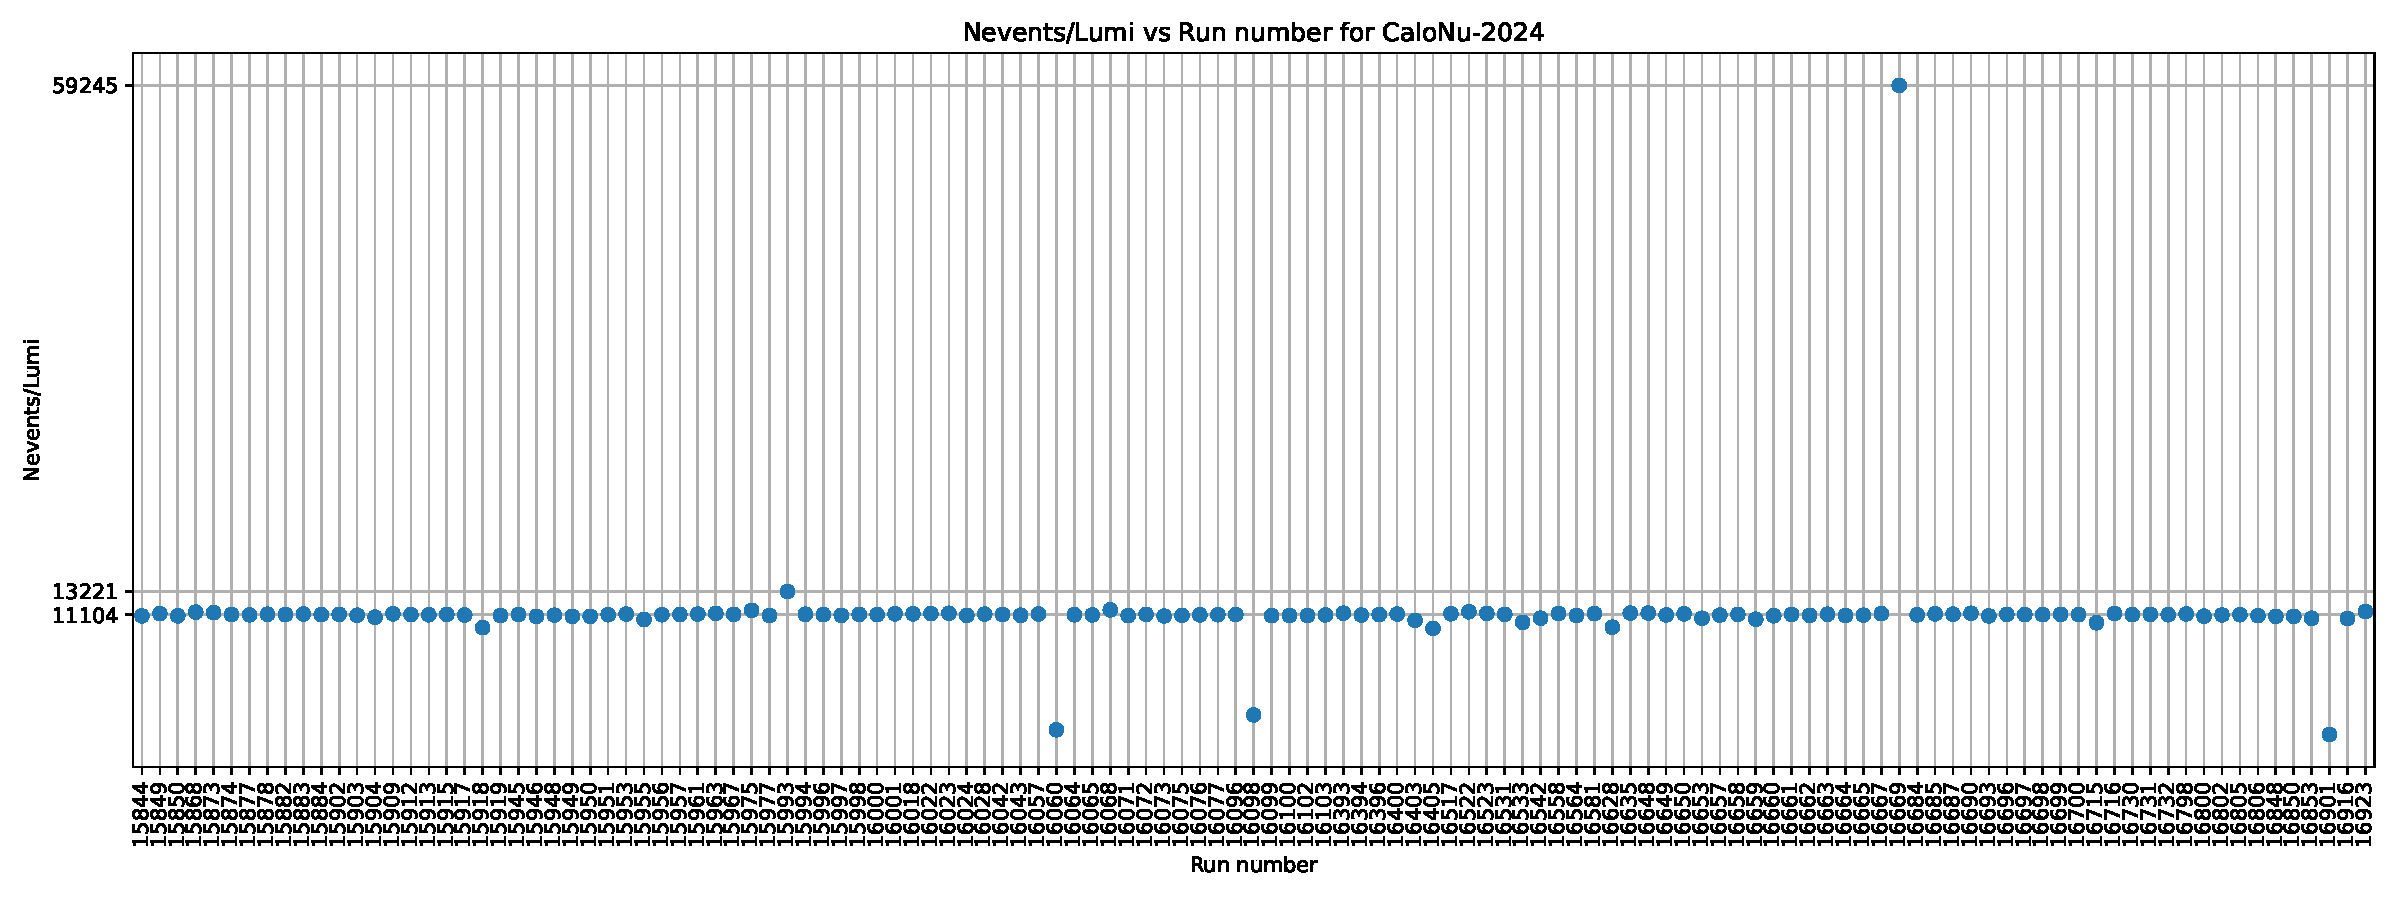
\includegraphics[width=1.0\textwidth]{plots_runwise/NEventsbyLumi_2024_CaloNu.pdf}
    \end{figure}
    \vspace{-0.35cm}
    \begin{figure}
        \centering
        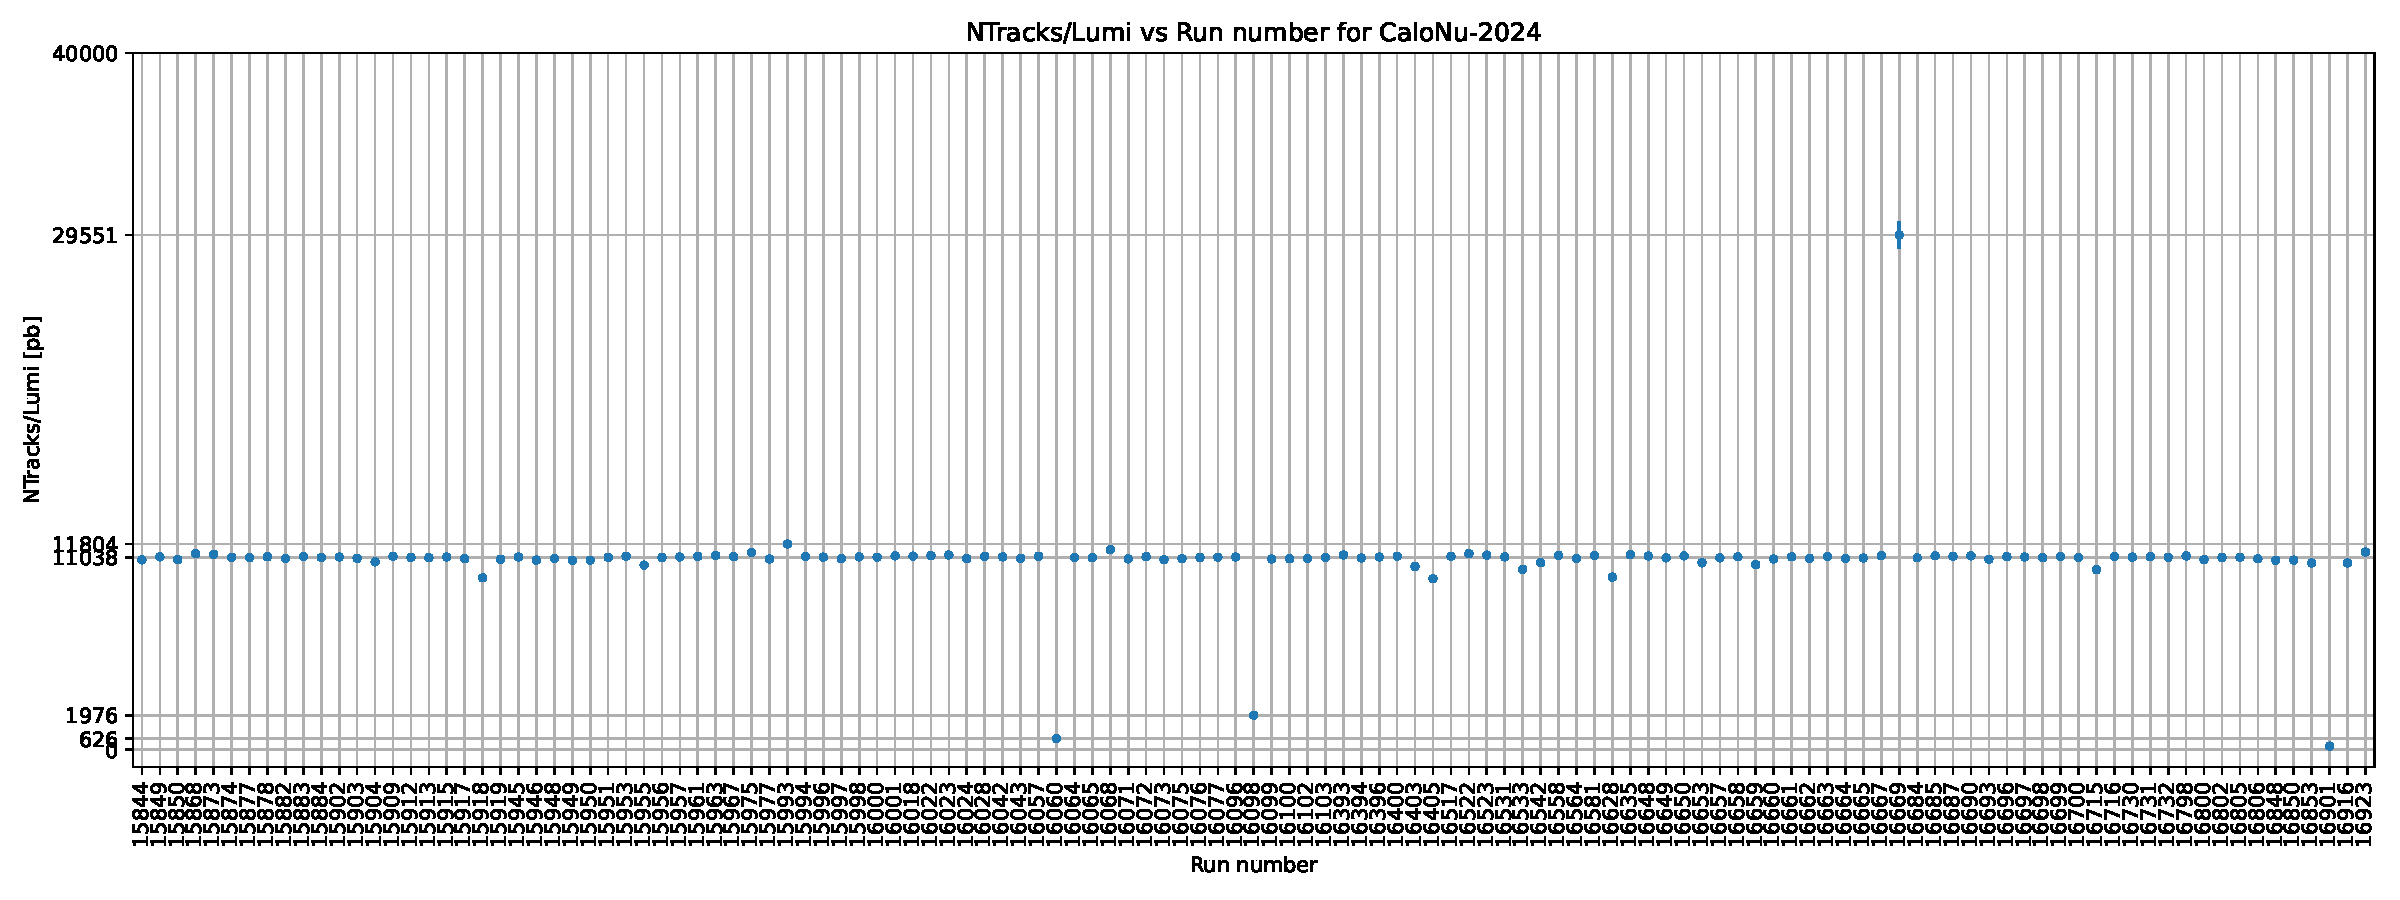
\includegraphics[width=1.0\textwidth]{plots_runwise/NTracksbyLumi_2024_CaloNu.pdf}
    \end{figure}
\end{frame}

\begin{frame}{Yield Plots of F243- 2024}
    \begin{figure}
        \centering
        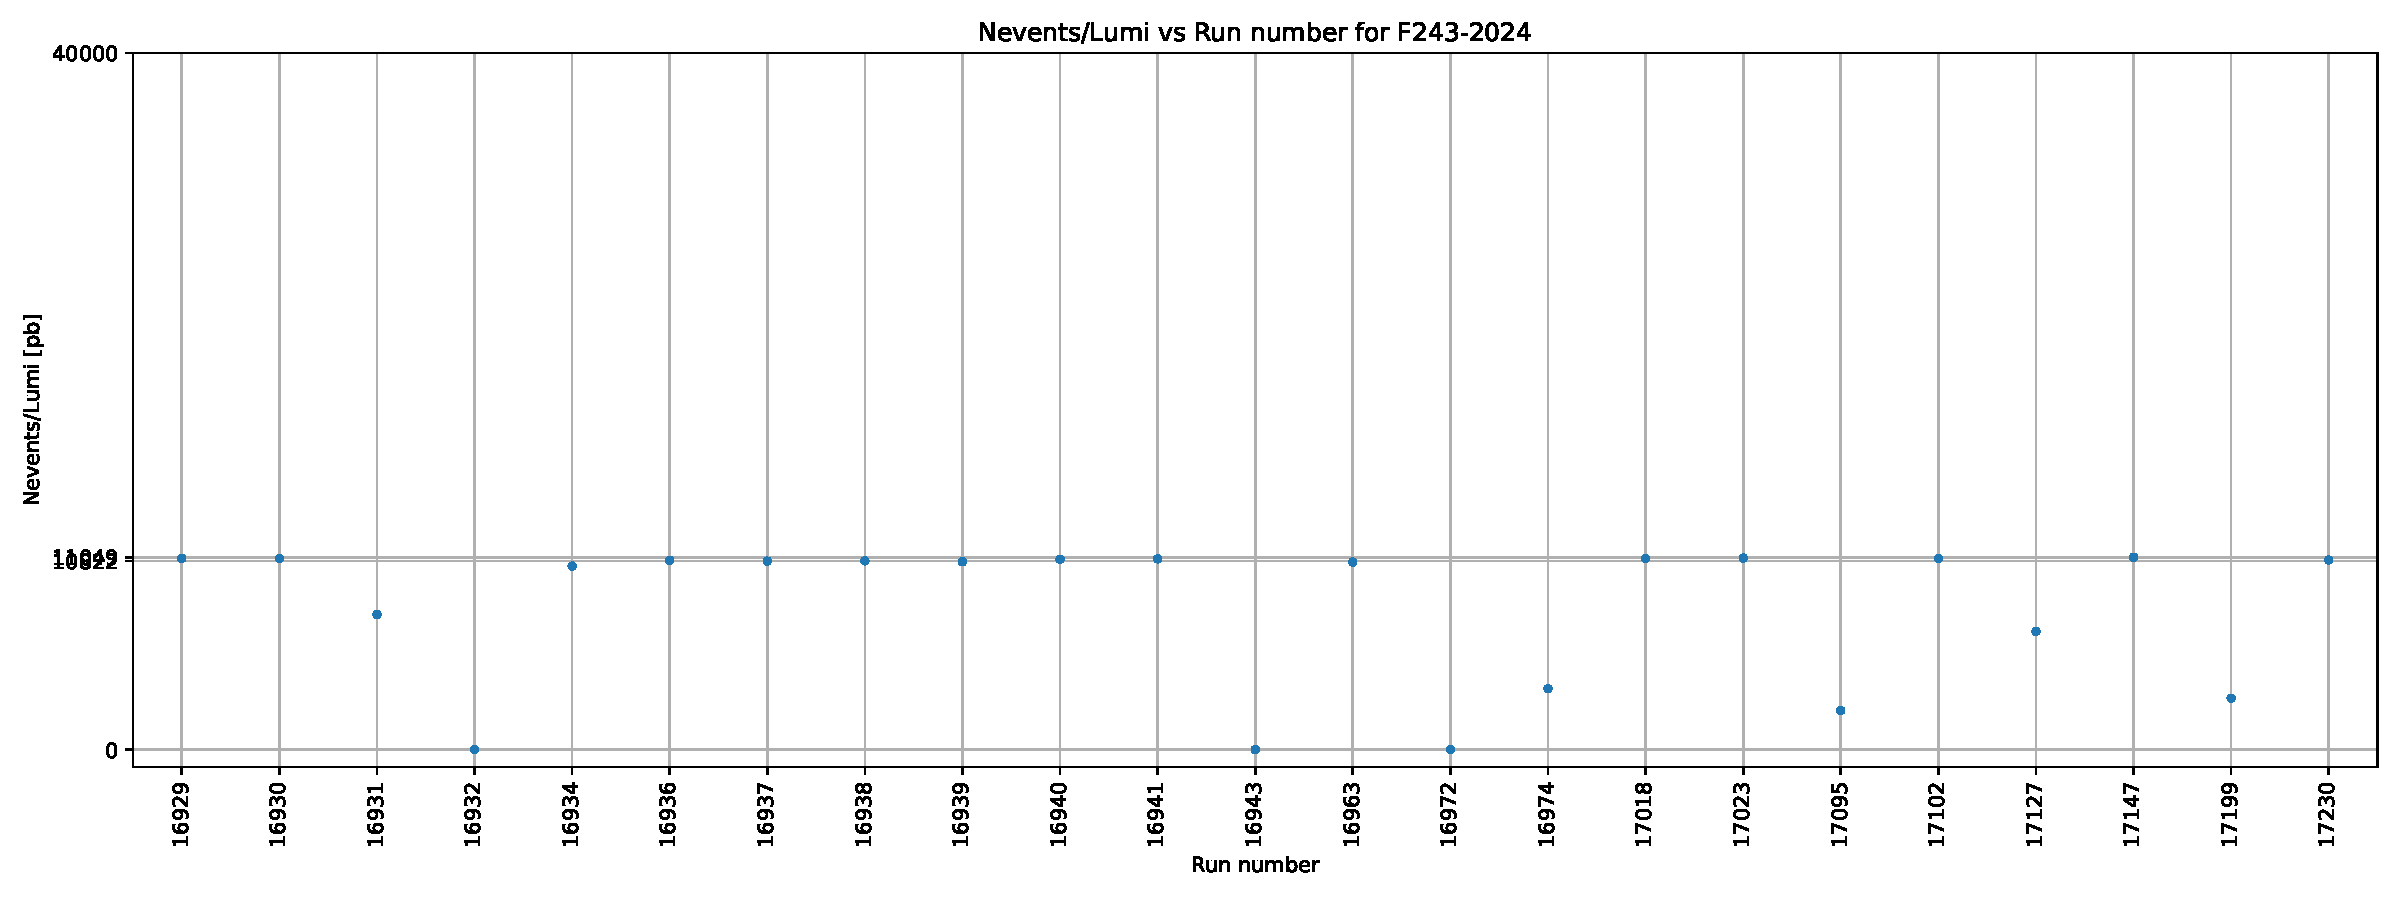
\includegraphics[width=1.0\textwidth]{plots_runwise/NEventsbyLumi_2024_F243.pdf}
    \end{figure}
    \vspace{-0.35cm}
    \begin{figure}
        \centering
        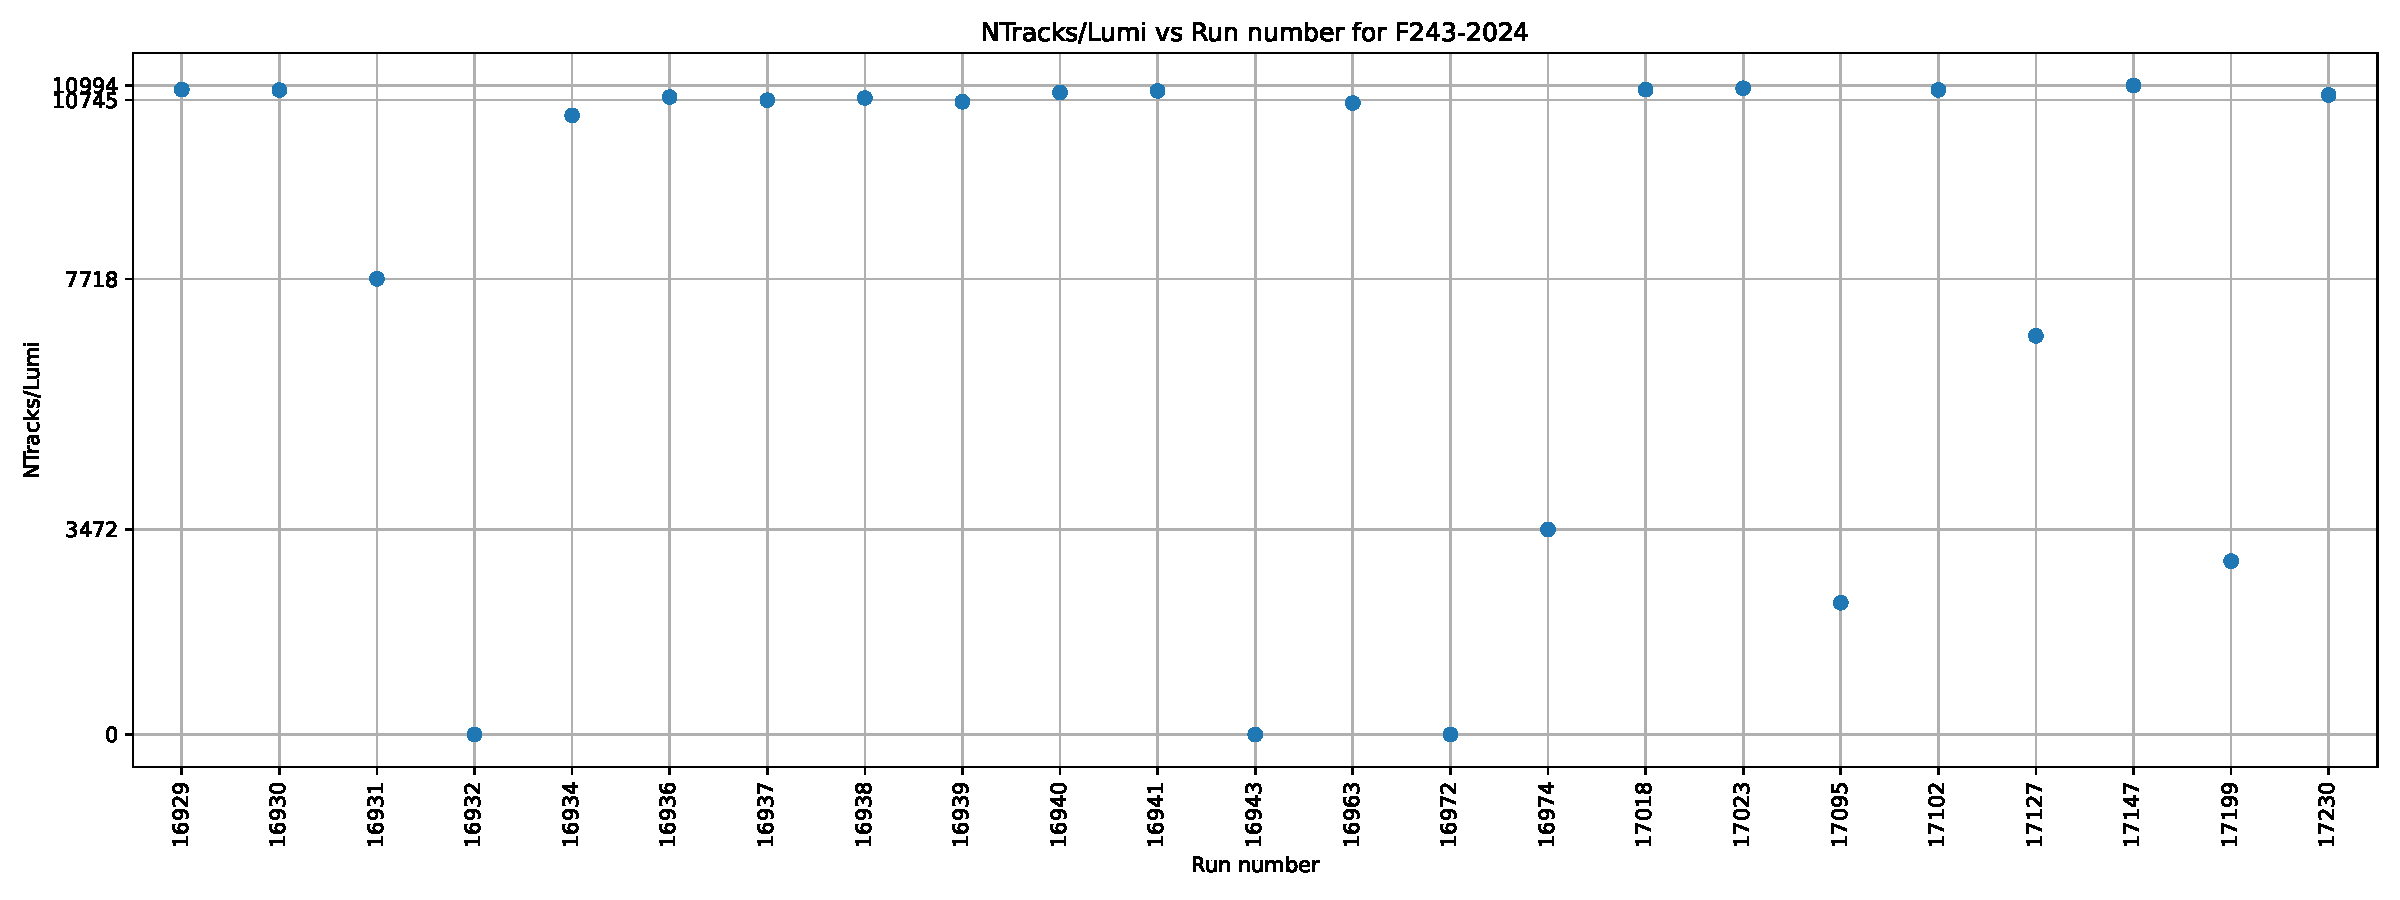
\includegraphics[width=1.0\textwidth]{plots_runwise/NTracksbyLumi_2024_F243.pdf}
    \end{figure}
\end{frame}

\begin{frame}{Yield Plots Summary}
    \begin{itemize}
        \item F241 - erratic behavior  during early runs 14587-14733
        \item Tungsten - erratic behavior for early to mid runs 15031-15267
        \item F242 - relatively stable except for 15676, 15694, 15814
        \item CaloNu - relatively stable expect for 16060, 16098, 1669, 16901
        \item F243 - low Nevent/lumi for 16931, 16974, 17095, 17127, 17147, 17199
        \item Some 0's in F243 artifact of empty ROOT files (16932, 16943, 16972)
    \end{itemize}
\end{frame}
\begin{frame}{Directions going Forward}
    \begin{itemize}
        \item Understand the DQ of other variables
        \item Investigate and understand the changes in Track Momenta
        \item Have a good run-list for the 2024 data (also for 2023)
        \item Investigate outliers in yield plots
        \item Investigate track variables as a function of run-splits in 2024
    \end{itemize}
\end{frame}
\begin{frame}{Micellaneous}
    \begin{itemize}
        \item Similar plots can be made using the \href{https://gitlab.cern.ch/anburger/compareproductions_faser}{compareproductions\_faser} tool. Some of the plots were used for validation.
        \item Link to Repo containing the code for plots in this presentation.
        \item Link to variants of the plots more more filtered like charge separated, good tracks only etc. [Will be added to above repo]
        \item Detailed yield plots were presented by Oscar. [See \href{https://indico.cern.ch/event/1476946/contributions/6220240/attachments/2970435/5227381/DQ2024.pdf}{DQ Talk}]
    \end{itemize}
\end{frame}
